% these are magic comments for TeXstudio
% !TeX program = xelatex
% !BIB program = biber

\documentclass[a4paper,12pt,twoside]{report}

%%% PACKAGES %%%

\usepackage{polyglossia}
\setdefaultlanguage[variant=uk]{english} % change to your language
%\setotherlanguage{czech} % if you need a specific part written in another language

% hyphenation rules for specialized words

%\AtBeginDocument{
%\hyphenation{pho-ton quan-tum}
%}

\usepackage{fontspec}

\usepackage[english=british]{csquotes}
\usepackage[xetex]{graphicx}

% see biblatex documentation
\usepackage[sorting=none,style=phys,backend=biber,defernumbers=true]{biblatex}
\usepackage[unicode]{hyperref}
\usepackage{xcolor}
\usepackage{amsmath}
\usepackage[font=small,labelfont=bf]{caption}
\usepackage{fancyhdr}
\usepackage{titlesec}
\usepackage{pdfpages}
\usepackage{microtype}
\usepackage{unicode-math}

% needed for a specific command changing bibliography formatting
\usepackage{xpatch}

% !!! LOREM IPSUM for demo purposes, you can get rid of this
\usepackage{lipsum}

% Libertinus fonts
\usepackage{libertinus-otf}

% At the moment, STIX looks better than Libertinus Math, but that will hopefully change soon.
% feel free to comment this out and try Libertinus Math
\setmathfont{STIX2Math.otf}

% if you like some extra ligaturesm enable this. Currently tt, tz, Th, ck, ch
% see libertinus repository on Github, file dhlig.fea

%\AtBeginDocument{
%\addfontfeatures{Ligatures=Discretionary}
%}

% metadata for the PDF file
\hypersetup{
pdfauthor={John Smith},
pdftitle={The Title of the Thesis},
pdfsubject={Typesetting},
pdfkeywords={Writing, academia, LaTeX, Libertinus}
}


%%% BIBLIOGRAPHY %%%

\addbibresource{thesis.bib}

% you may put the publications you authored in a separate category
\DeclareBibliographyCategory{MyArticles}
\addtocategory{MyArticles}{Smith2017}

% force the order you want
\nocite{Smith2017}

%%% BIBLATEX OPTIONS AND TWEAKS %%%

% Biblatex enables editing .bib entries and configuring everything in your LaTeX document

% get rid of the months
\DeclareSourcemap{
  \maps[datatype=bibtex]{
    \map[overwrite]{
      \step[fieldset=month, null]
    }
  }
}

% declare special bibliography contexts with optional prefixes
\DeclareRefcontext{myarticles}{labelprefix=A}
\DeclareRefcontext{books}{labelprefix=B}

% change the typesetting of reference numbers in the bibliography

\DeclareFieldFormat{labelnumberwidth}{#1\hspace{10pt}}

% declare command \citenum that prints a plain reference number
% can be used in a sentence

\DeclareCiteCommand{\citenum}
  {\printtext[bibhyperref]{\printfield{labelprefix}}}
  {\printtext[bibhyperref]{\printfield{labelnumber}}}
  {}
  {}

% produce clickable URL links for theses
\letbibmacro{ORIG-institution+location+date}{institution+location+date}
\renewbibmacro*{institution+location+date}
{\iffieldundef{url}
		{\usebibmacro{ORIG-institution+location+date}}
		{\href{\thefield{url}}{\usebibmacro{ORIG-institution+location+date}}}
}

% small caps typesetting of author names
\DeclareNameWrapperFormat{author}{\textsc{#1}}

% make the 'and' between the last two authors upright and not small caps
% taken from biblatex.def and modified
\DeclareDelimFormat{finalnamedelim}{
\textup{
  \ifnumgreater{\value{liststop}}{2}{\finalandcomma}{}%
  \addspace\bibstring{and}\space
  }
}

% after the authors list, there is a colon and a newline
\renewcommand{\labelnamepunct}{\addcolon\newline}

% the newline between name and journal is tricky to add, because there is no command to redefine.
% here is some black magic using the package xpatch
% taken from https://tex.stackexchange.com/questions/351397/biblatex-add-line-breaks-after-author-and-title
\makeatletter
\def\do#1{
  \ifcsdef{blx@bbx@#1}
    {\xpatchbibdriver{#1}
       {\printlist{language}%
        \newunit\newblock}
       {\printlist{language}%
        \printunit{\addcomma\newline}}
       {}{}}
    {}} 
\abx@doentrytypes
\makeatother

% make the font size smaller for bibliography
\renewcommand*{\bibfont}{\footnotesize}
 
% if you don't like titles in quotes, this gets rid of them

%\DeclareFieldFormat[article,inproceedings,patent,incollection]{title}{%
%  \iftoggle{bbx:chaptertitle}
%    {#1\isdot}
%    {}%
%}




%%% PAGE HEADERS AND FOOTERS %%%

% !!! the narrow margins are inner margins, while the wider margins are outer margins
% odd-numbered pages  1,3,5,... right side >>> __text____
% even-numbered pages 2,4,6,... left side  >>> ____text__
% see https://en.wikipedia.org/wiki/Canons_of_page_construction

% page layout and margins are left at default settings

\pagestyle{fancy}

% this is here only so LaTeX does not complain
\setlength{\headheight}{15pt}

% the aim here is to have section names in the headings on the inner side
% the way I think this works is:
% when evaluating the \section[shortName]{fullName} command in the text, there is a \sectionmark command inside.
% calling \markboth like below changes the current heading to shortName
% works the same for chapters, both commands are redefined to cover the cases where the chapter does not contain a section immediately
% !!! asterisk commands and table of contents do not contain marks, so you need to do it manually (see the main text)
\renewcommand{\chaptermark}[1]{\markboth{\textsc{#1}}{}}
\renewcommand{\sectionmark}[1]{\markboth{\textsc{#1}}{}}

% remove page numbers from the footer and put it into the header (outer side)
\fancyfoot{}
\fancyhf[HLE,HRO]{\thepage}

% redefine plain style to be compatible with fancy (beginning of chapters)
\fancypagestyle{plain}{ %
  \fancyhf{} % remove everything
  \renewcommand{\headrulewidth}{0pt} % remove lines as well
  \renewcommand{\footrulewidth}{0pt}
}


%%% MISCELLANEOUS %%%

% hyperlinks are highlighted using colored text instead of colored boxes
% !!! switch off for printing unless you want the color in print

\hypersetup{
    colorlinks,
    linkcolor={red!50!black},
    citecolor={blue!80!black},
    urlcolor={blue!80!black}
}


% heading styles, sans serif

\def\headingStyle{\sffamily}

\titleformat*{\section}{\LARGE\headingStyle}
\titleformat*{\subsection}{\Large\headingStyle}
\titleformat*{\subsubsection}{\large\headingStyle}
\titleformat{\chapter}[display]
{\huge\headingStyle}{\chaptertitlename\ \thechapter}{20pt}{\Huge\headingStyle}

% in case you like prefixes to distinguish tables and figures from other numbered references

%\renewcommand{\thefigure}{F\arabic{chapter}.\arabic{figure}}
%\renewcommand{\thetable}{T\arabic{chapter}.\arabic{table}}


%%%%%%%%%%%%%%%%%%%%%%%%%%%%%%%%%%%%%%%%%%%%%%%%%%%%%%%%%%%%%%%%%%%%%

\begin{document}

\pagenumbering{roman}
\pagestyle{empty}

% LaTeX is not an efficient tool for visual typesetting, so the title page is done in Inkscape

\includepdf{title_page.pdf}

\centerline{\headingStyle\Large Abstract}

\bigskip
\noindent

Abstract goes here.

\lipsum[1]

\vfil

\noindent\textbf{Keywords:} keywords

\vfil

{\centering
\begin{tabular}{rl}
Title: & The Title of the Thesis	\\
 & That Might Be Too Long For One Line	\\
Author: & John Smith	\\
Advisor: & Harry Jones	\\
Study programme: & Typesetting	\\
Institution: & Department of Typography, Splendid University\\
Year: & 2019	\\
Pages: & 100
\end{tabular}
}

\vfil
\noindent
Legal and other disclaimers.

\lipsum[2]

\clearpage


\mbox{}
\vfil

\centerline{\headingStyle\Large Acknowledgements}

\bigskip

\noindent
Here I thank everyone who helped me while I was working on my thesis.

\lipsum[3-4]

\vfil

\clearpage

\pagestyle{fancy}

\tableofcontents
\markboth{\textsc{Contents}}{}

\chapter*{Preface}
\addcontentsline{toc}{chapter}{Preface}
\markboth{\textsc{Preface}}{}

% this part may be included from a separate file by \input

Here I explain my contribution to the thesis and how it came to be.

\lipsum[1-4]

\lipsum[6-8]

\vspace{1cm}

\noindent
\parbox{.4\textwidth}{
Hometown
\\
April 2019
}
\hfill
\parbox{.4\textwidth}{\flushright
John Smith
\\
j.smith@splendid-uni.org
}

\clearpage
\pagestyle{empty}
\cleardoublepage

\pagenumbering{arabic}
\pagestyle{fancy}

%%% MAIN TEXT BEGINS %%%
% it is best to have chapters in separate files and include them by \input

\chapter{Introduction}
\label{chapter.intro}

This is an intro.\autocite{Smith2017} It may cite some references.\autocite{Migdall2013Book,Straka2014,Straka2018Apr,Straka2019Thesis} Reference \citenum{Straka2019Thesis} is the original thesis typeset using this template.

\lipsum[1-4]

\lipsum[6-9]

\lipsum[11-12]

\chapter{Content}

\section{The first section}

A picture is included in Figure \ref{fig}. Equations \eqref{SPDC.state} to \eqref{math.PoissonBayes} show some math. Thanks to the package \textsc{unicode-math}, you can insert Unicode mathematical symbols directly into the \LaTeX{} code.

\begin{align}\label{SPDC.state}
\left| \text{\sc SPDC} \right> &\approx \left| \text{vac.} \right> + \iint\limits_{\mathbf{k}_1,\mathbf{k}_2} \varPsi(\mathbf{k}_1,\mathbf{k}_2)a^\dagger_{\mathbf{k}_1}a^\dagger_{\mathbf{k}_2} \left|\text{vac.} \right>.
\\
\text{DFT}(f)_s &= \sum_{r=0}^{n-1} f_r e^{-2\pi r s/n},
\\
g^{(2)}(0) &\coloneq \frac{\langle n(n-1) \rangle}{\langle n \rangle^2} \approx \frac{2 p_2}{p_1^2} \approx \mathcal{R}\tau_c (2-\eta_t).
\\
\label{math.PoissonBayes}
P(\theta|N_m) &= \lim_{U \rightarrow \infty} \left( \frac{\frac{\theta^{N_m}}{N_m!} e^{-\theta} \cdot \frac{1}{U}}{\int_0^U \frac{\theta^{N_m}}{N_m!} e^{-\theta} \cdot \frac{1}{U}\,\text{d}\theta} \right) = \frac{\theta^{N_m}}{N_m!} e^{-\theta}.
\end{align}

\lipsum[1-2]

\begin{figure}
\centering
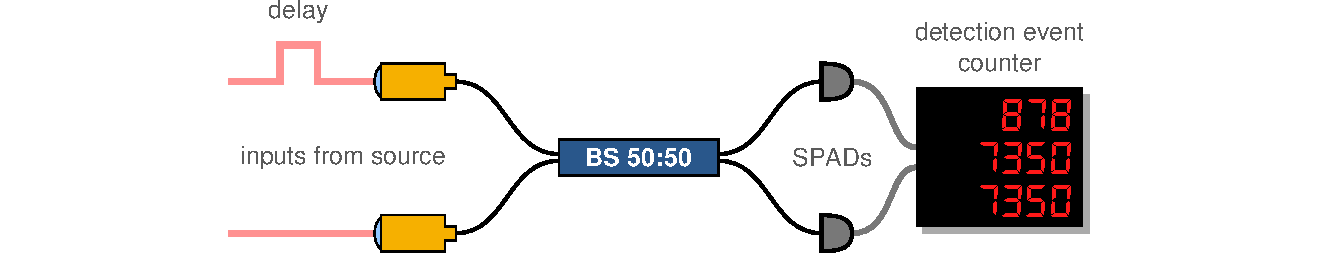
\includegraphics[width=\linewidth]{figure.pdf}
\caption{This shows a measurement scheme.\autocite{Straka2019Thesis}}
\label{fig}
\end{figure}


\lipsum[3-4]

\lipsum[6-9]

\lipsum[14-20]

\section[The second section]{The second section with a very long title that would not fit in the header}

\lipsum[19-30]

%%% REFERENCES %%%

\defbibheading{bibliography}[\bibname]{
	\chapter*{References}
	\addcontentsline{toc}{chapter}{References}
	\markboth{\textsc{References}}{}
}

\printbibheading
\newrefcontext{myarticles}
\printbibliography[heading=subbibliography,resetnumbers,category=MyArticles,title={Articles covering the presented results}]
\newrefcontext{books}
\printbibliography[heading=subbibliography,resetnumbers,type=book,title={Books}]
\newrefcontext{nonbooks}
\printbibliography[heading=subbibliography,resetnumbers,nottype=book,notcategory=MyArticles,title={Articles, proceedings and theses}]



\end{document}